\chapter{The Equivalence Mapping}
\label{chap:equiv_mapping}

Another question that is worth getting into is the following. Say we are given two transducers $\cT_1$ and $\cT_2$ such that $\cT_1 \prec_{k} \cT_2$, and an input word $x\in \left(\Sigma^k\right)^\star$. This means, of course, that there is a way to permute the rounds in $x$ to obtain a matching word $x'$ for $\cT_2$.
Consider the mapping $\psi_{\cT_1,\cT_2}: x\mapsto x'$ that maps every input word $x$ to a corresponding permutation $x'$ (and we drop the subscript when the transducers are implied from the context). We call this the \emph{equivalence mapping}. What can we say about it? Specifically, is it regular? We begin with an example.

\begin{example}
\label{example:mapping}

Let $\sI=\{a,b\}$, $\sO=\{0,1\}$ and $\cT_1$ be a transducer that expects to see either $ab$ or $ba$ in every round, outputting $00$ in both cases, and otherwise outputs $01$ in that round. Let also $\cT_2$ be a transducer that expects the first round to be $ab$ and the second to be $ba$, otherwise outputs $01$ in the round not meeting expectations; and beginning from the third round, it behaves like $\cT_1$ (see~\autoref{fig:example_mapping}). We have that $\cT_1\prec_{2}\cT_2$ by a permutation that corrects the order of the letters in the first two rounds of the input. Moreover, we have $\psi(ab)= \psi(ba)=ab$ whereas $\psi(abba)=abba \neq \psi(ab) \cdot \psi(ba)$.

\begin{figure}[ht]
	\centering
	\begin{tikzpicture}[shorten >=1pt,node distance=1.5cm and 1.5cm,on grid,auto]
	    \tikzset{every state/.style={minimum size=7mm}};
	    \node[state] (q'_i) [initial above, text=red, fill=blue!10] {$0$};
        \node[state] (q'_ab) [right=of q'_i, text=red, fill=blue!10] {$0$};
        \node[state] (q'_ba) [below=of q'_i, text=red, fill=blue!10] {$0$};
        \node[state] (q'_f) [below=of q'_ab, text=red, fill=blue!10] {$1$};
        \path[->] 
        (q'_i)  edge [bend left=10] node {$a$} (q'_ab)
        (q'_i)  edge [bend left=10] node {$b$} (q'_ba)
        (q'_ab) edge [bend left=10] node {$a$} (q'_f)
        (q'_ab) edge [bend left=10] node {$b$} (q'_i)
        (q'_ba) edge [bend left=10] node {$a$} (q'_i)
        (q'_ba) edge [bend left=10] node {$b$} (q'_f)
        (q'_f)  edge [bend left=10] node {$a$} (q'_ab)
        (q'_f)  edge [bend left=10] node {$b$} (q'_ba);
	    
        \node[state] (q_0) [initial above, right=of q'_ab, text=red] {};
        \node[state] (q1_a) [right=of q_0, text=red, fill=red!10] {$0$};
        \node[state] (q1_b) [below right=of q_0, text=red, fill=red!10] {$0$};
        \node[state] (q1_ab) [right=of q1_a, text=red, fill=red!10] {$0$};
        \node[state] (q1_ba) [right=of q1_b, text=red, fill=red!10] {$1$};
        \node[state] (q2_b) [right=of q1_ab, text=red, fill=green!10] {$0$};
        \node[state] (q2_a) [right=of q1_ba, text=red, fill=green!10] {$0$};
        \node[state] (q2_ba) [right=of q2_b, text=red, fill=green!10] {$0$};
        \node[state] (q2_ab) [right=of q2_a, text=red, fill=green!10] {$1$};
        \node[state] (q_i) [right=of q2_ba, text=red, fill=blue!10] {$0$};
        \node[state] (q_ab) [right=of q_i, text=red, fill=blue!10] {$0$};
        \node[state] (q_ba) [right=of q2_ab, text=red, fill=blue!10] {$0$};
        \node[state] (q_f) [right=of q_ba, text=red, fill=blue!10] {$1$};
        \path[->] 
        (q_0)   edge [] node {$a$} (q1_a)
        (q_0)   edge [sloped, pos=0.2] node {$b$} (q1_b)
        (q1_a)  edge [sloped, pos=0.2] node {$a$} (q1_ba)
        (q1_a)  edge [] node {$b$} (q1_ab)
        (q1_b)  edge [] node {$a,b$} (q1_ba)
        (q1_ab) edge [sloped, pos=0.2] node {$a$} (q2_a)
        (q1_ab) edge [] node {$b$} (q2_b)
        (q1_ba) edge [] node {$a$} (q2_a)
        (q1_ba) edge [sloped, pos=0.2] node {$b$} (q2_b)
        (q2_a)  edge [] node {$a,b$} (q2_ab)
        (q2_b)  edge [] node {$a$} (q2_ba)
        (q2_b)  edge [sloped, pos=0.2] node {$b$} (q2_ab)
        (q2_ab) edge [out=-30, in=-50, sloped, looseness=2, below] node {$a$} (q_ab)
        (q2_ab) edge [] node {$b$} (q_ba)
        (q2_ba) edge [out=30,in=140, sloped] node {$a$} (q_ab)
        (q2_ba) edge [sloped, pos=0.2] node {$b$} (q_ba)
        (q_i)   edge [bend left=10] node {$a$} (q_ab)
        (q_i)   edge [bend left=10] node {$b$} (q_ba)
        (q_ab)  edge [bend left=10] node {$a$} (q_f)
        (q_ab)  edge [bend left=10] node {$b$} (q_i)
        (q_ba)  edge [bend left=10] node {$a$} (q_i)
        (q_ba)  edge [bend left=10] node {$b$} (q_f)
        (q_f)   edge [bend left=10] node {$a$} (q_ab)
        (q_f)   edge [bend left=10] node {$b$} (q_ba);
    \end{tikzpicture}
	\caption{The transducers $\cT_1$ (left) and $\cT_2$ (right) in \autoref{example:mapping}. The states of $\cT_2$ in red, green and blue manage the first, second and later rounds, respectively.}
	\label{fig:example_mapping}
\end{figure}
\end{example}

The above example shows that $\psi$ is not a homomorphism: it does not satisfy $\psi(xy)=\psi(x)\psi(y)$. Next, we show that $\psi$ cannot be described by a look-ahead machine. We use an example of round simulation with restriction; however, we have tested and confirmed that it is possible to get rid of the restriction language $\Lambda$. Moreover, the example uses a round length of $k=3$, but it can be extended to any round length $k>0$ in a similar manner.

\begin{example}
\label{example:lookahead}
Set $\Lambda=L[ab\cdot (cc)^\star\cdot (ab+ba)]$ and $k=2$, and let $\cT_1$ and $\cT_2$ be the transducers in~\autoref{fig:example_lookahead}, satisfying $\cT_1\prec_{k,\Lambda} \cT_2$. Denote the equivalence mapping by $\psi^\star: (\Sigma_I^k)^\star \rightarrow (\Sigma_I^k)^\star$.

\begin{figure}[ht]
	\centering
	\begin{tikzpicture}[shorten >=1pt,node distance=1.5cm and 1.5cm,on grid,auto]
	    \tikzset{every state/.style={minimum size=7mm}};
	    \node[state] (q_0)  [initial above, text=red] {};
        \node[state] (q_a) [right=of q_0, text=red] {$1$};
        \node[state] (q_b) [below=of q_a, text=red] {$1$};
        \node[state] (q'_0) [right=of q_a, text=red, fill=orange!20] {$2$};
        \node[state] (q'_a) [right=of q'_0, text=red] {$3$};
        \node[state] (q'_b) [below=of q'_a, text=red] {$5$};
        \node[state] (q'_ab) [right=of q'_a, text=red] {$4$};
        \node[state] (q'_ba) [right=of q'_b, text=red] {$6$};
        \path[->] 
        (q_0)  edge [] node {$a$} (q_a)
        (q_0)  edge [sloped] node {$b$} (q_b)
        (q_a) edge [] node {$b$} (q'_0)
        (q_b) edge [sloped] node {$a$} (q'_0)
        (q'_0) edge [loop above] node {$c$} (q'_0)
        (q'_0) edge [] node {$a$} (q'_a)
        (q'_0) edge [sloped] node {$b$} (q'_b)
        (q'_a) edge [] node {$b$} (q'_ab)
        (q'_b) edge [] node {$a$} (q'_ba);
    \end{tikzpicture}%
    \hspace{1.5cm}%
	\begin{tikzpicture}[shorten >=1pt,node distance=1.5cm and 1.5cm,on grid,auto]
	    \tikzset{every state/.style={minimum size=7mm}};
	    \node[state] (q_0)  [initial above, text=red] {};
        \node[state] (q_a) [right=of q_0, text=red] {$1$};
        \node[state] (q_b) [below=of q_a, text=red] {$1$};
        \node[state] (q'_0) [right=of q_a, text=red, fill=orange!20] {$2$};
        \node[state] (q'_1) [right=of q_b, text=red, fill=orange!20] {$2$};
        \node[state] (q'_a) [right=of q'_0, text=red] {$3$};
        \node[state] (q'_b) [below=of q'_a, text=red] {$5$};
        \node[state] (q'_ab) [right=of q'_a, text=red] {$4$};
        \node[state] (q'_ba) [right=of q'_b, text=red] {$6$};
        \path[->] 
        (q_0)  edge [] node {$a$} (q_a)
        (q_0)  edge [sloped] node {$b$} (q_b)
        (q_a) edge [] node {$b$} (q'_0)
        (q_b) edge [] node {$a$} (q'_1)
        (q'_0) edge [loop above] node {$c$} (q'_0)
        (q'_1) edge [loop above] node {$c$} (q'_1)
        (q'_0) edge [] node {$a$} (q'_a)
        (q'_1) edge [] node {$b$} (q'_b)
        (q'_a) edge [] node {$b$} (q'_ab)
        (q'_b) edge [] node {$a$} (q'_ba);
    \end{tikzpicture}
	\caption{Something about \autoref{example:lookahead}.}
	\label{fig:example_lookahead}
\end{figure}

We claim that for any $r$, there exists no look-ahead machine that defines a function $\psi_r: (\Sigma_I^{rk})^\star \rightarrow (\Sigma_I^{rk})^\star$ such that $\psi^\star(x)=\psi(x)$ for all input words $x$.

Indeed, let $r$ be given, and assume by contradiction that such $\psi_r$ exists. Now consider the input word $x=ab\cdot c^{rk-2}$. $\psi_r(x)$ must start with either $ab$ or $ba$. Without loss of generality, assume the former, and consider the input word $x':=x\cdot ba\cdot c^{rk-2}$. $\psi_r$ works on $r$ rounds each time, so that the first $r$ rounds are fixed when it reads the $(r+1)$-th round. Since $\psi_r(x')$ must induce a valid path in $\cT_2$, the only option for the $(r+1)$-th round of $\psi_r(x')$ is $ab$. Hence, the output of $\cT_1$ on $x'$ is different from the output of $\cT_2$ on $\psi(x')$, and we have a contradiction.
\end{example}

% This example only works if we assume that $\psi_r$ is ``ignorant'' of the fact that, actually, we will \emph{never} want to shuffle the very first round to be $ba$. This is a piece of knowledge so simple that it might not be practically reasonable to have it hidden from $\psi_r$.

% The example can be extended to any round length $k$; and it is possible to get rid of the restriction language $\Lambda$, as well. See the generalized transducers below (``Dec 21$^\text{st}$'').

We saw that a look-ahead (actually, a ``compound'' of rounds or part-rounds) of $r$ rounds does not work, for any $r$. Also, it is clear that a look-ahead of a number not divisible by $k$ will not work either, since we must at least read the whole round to know the correct way to shuffle. Hence, no look-ahead machine can define $\psi^\star$.

A sliding-window variation of the former, in which at any given round, we can see $r-1$ additional rounds in the future, would not work either, with the same counter-example. Indeed, even if we know the future beforehand, it does not permit us to rewrite the past, so a wrong choice in the first round would not be fixed.

In fact, it would be possible to effectively ``rewrite'' the past by permitting delayed output. A finite-state machine supporting delayed output would be enough for the $\psi^\star$ of the last example: the machine would read the input round-by-round, searching for two rounds of the form $a^{k-2}\left(ab+ba\right)$ (not necessarily consecutive). Once they are detected, it would decide the output for the \emph{first} of them according to the second. Deciding the remainder of the output is simple.

% 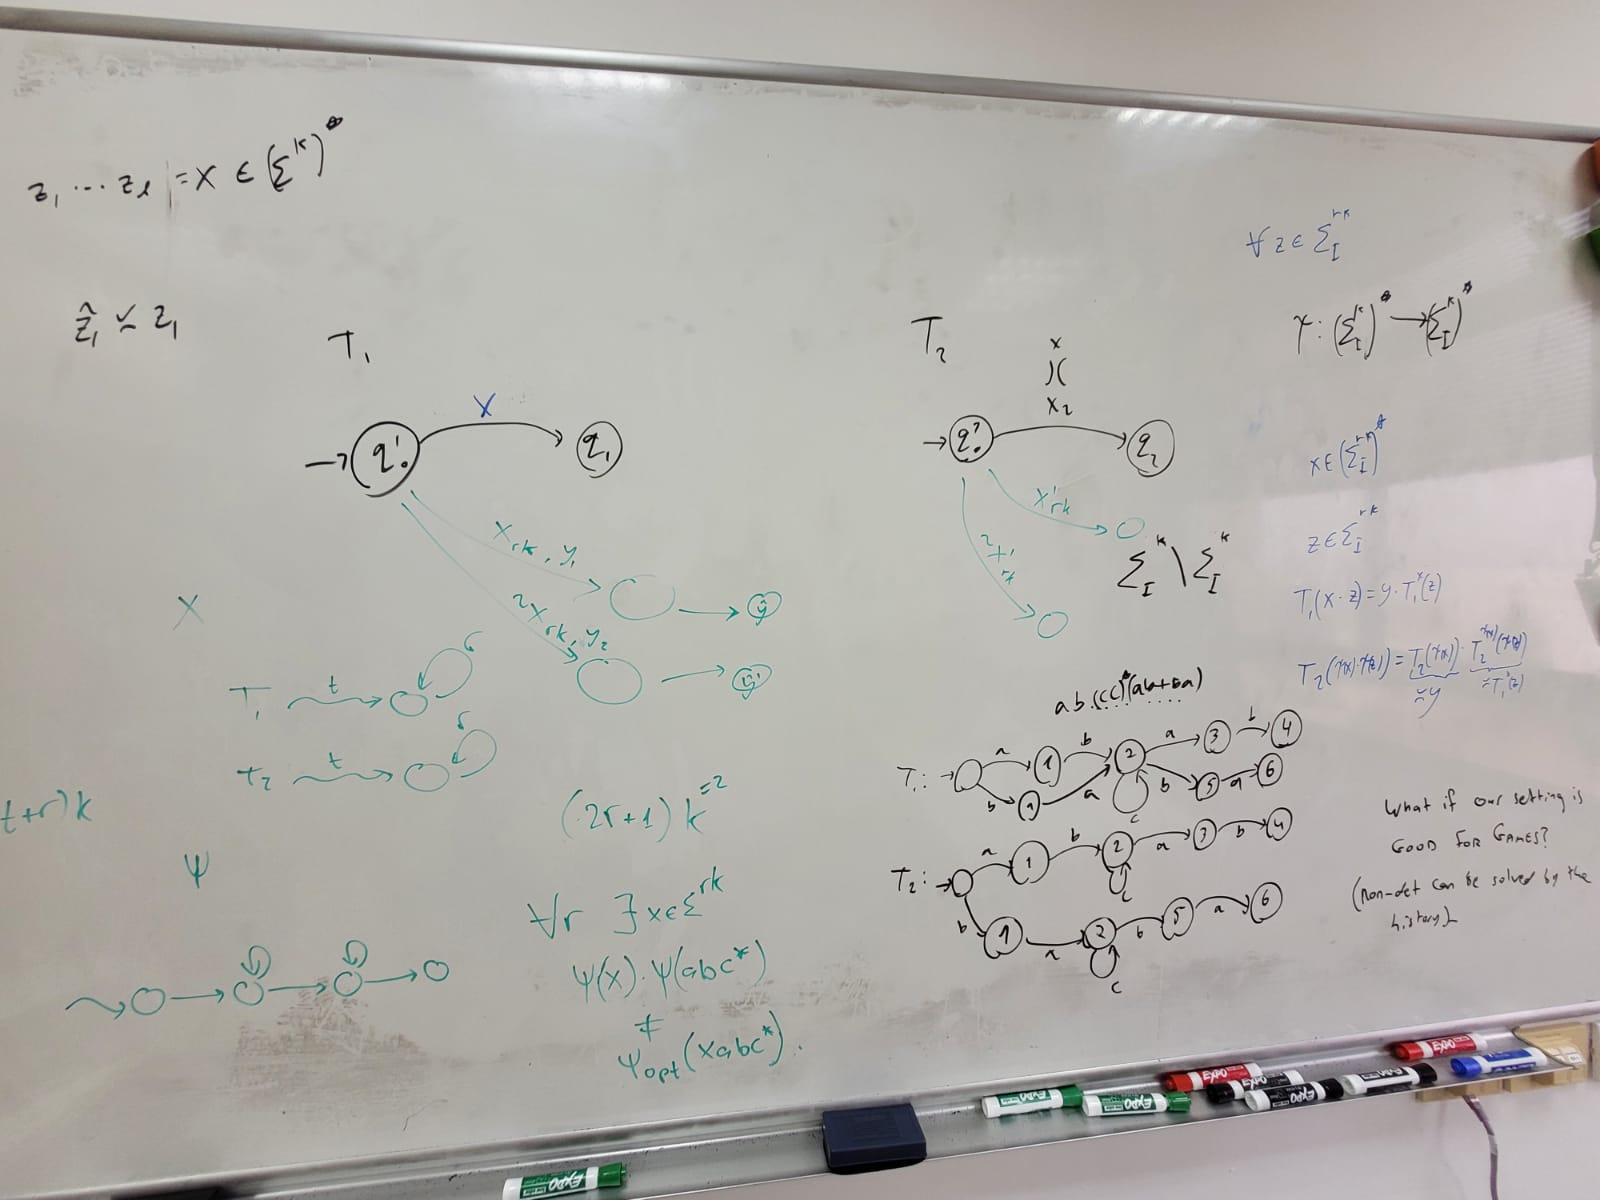
\includegraphics[width=\linewidth]{graphics/wb6.jpg}
% 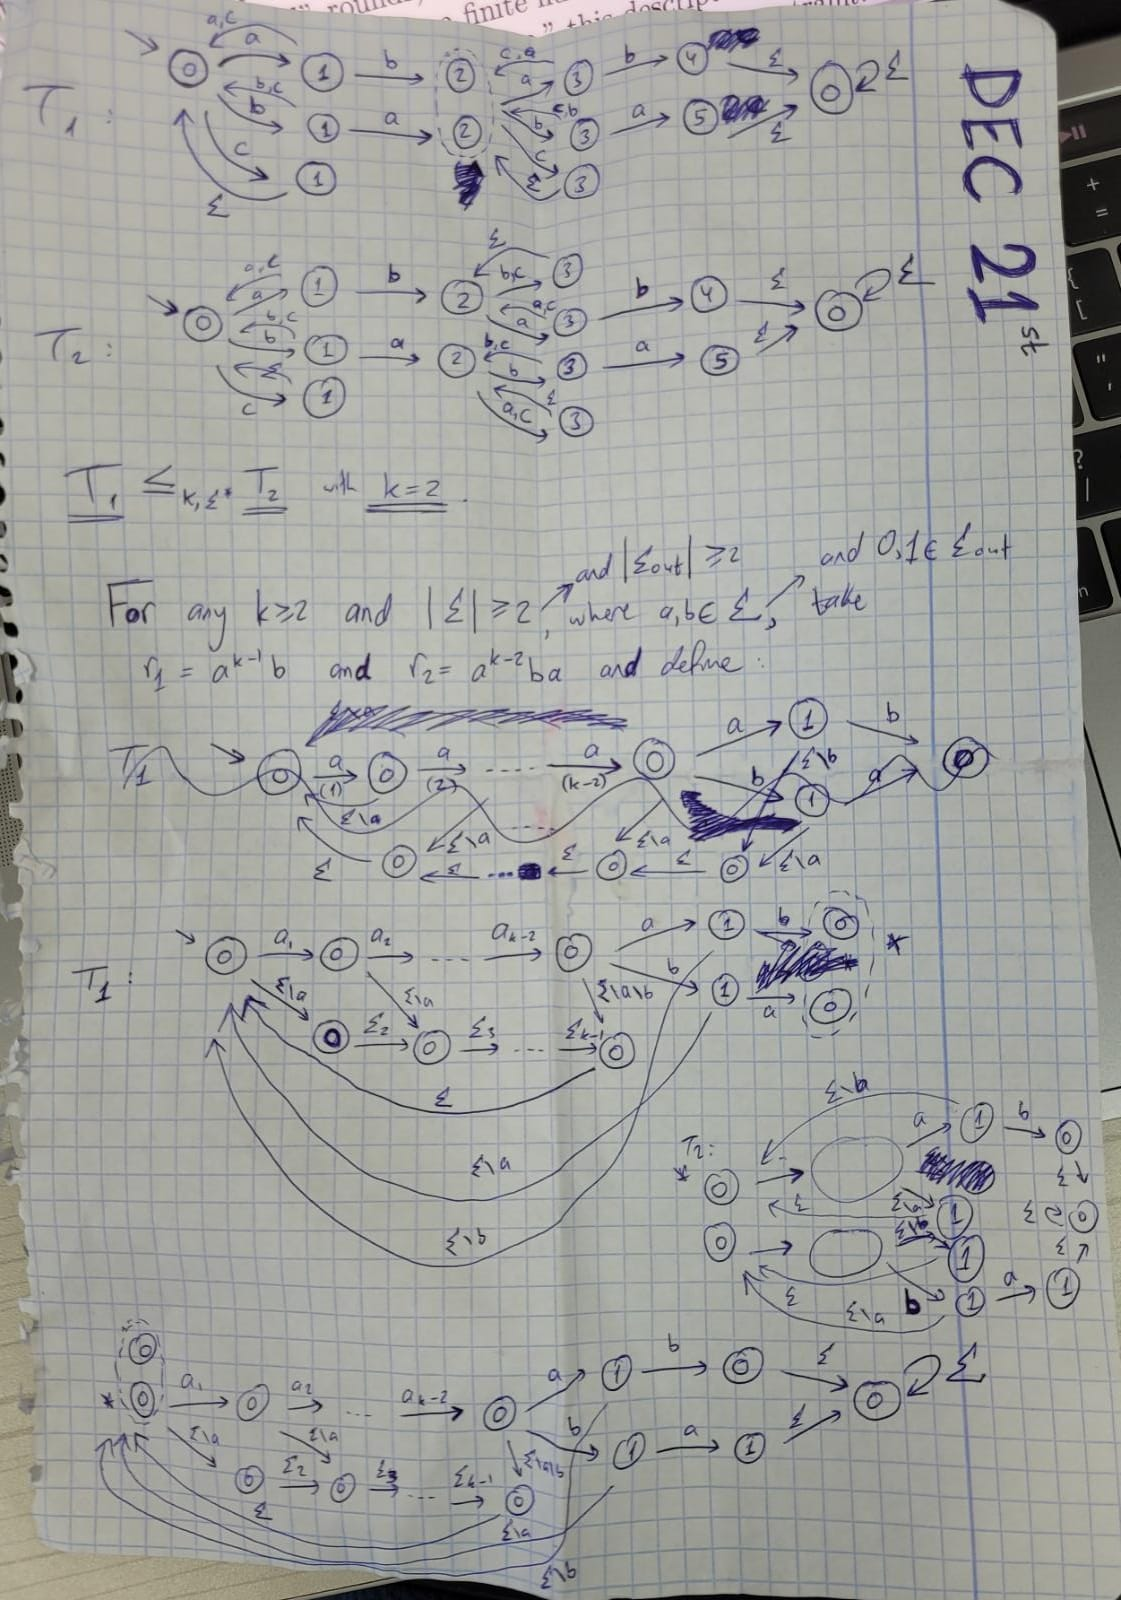
\includegraphics[width=\linewidth]{graphics/dec21.jpeg}
